\documentclass{article}
%\usepackage[latin1]{inputenc}
\usepackage[spanish]{babel}
\usepackage{amsfonts}
\usepackage{amsmath}
\usepackage{graphicx}
\usepackage{url}
\usepackage[top=3cm,bottom=3cm,left=3.5cm,right=3.5cm,footskip=1.5cm,headheight=1.5cm,headsep=.5cm,textheight=3cm]{geometry}
\usepackage{float}
\usepackage{algorithm}
\usepackage{algpseudocode}
\usepackage{ mathrsfs }

\makeatletter
  \renewcommand{\ALG@name}{Algoritmo}
\makeatother

\begin{document}
\title{Inteligencia Artificial \\ \begin{Large}Informe Final: Problema Risk-constrained Cash-in-Transit Vehicle Routing Problem\end{Large}}
\author{Sofía Riquelme}
\date{\today}
\maketitle


%--------------------No borrar esta secci\'on--------------------------------%
\section*{Evaluaci\'on}

\begin{tabular}{ll}
C\'odigo Fuente (20\%): &  \underline{\hspace{2cm}}\\
Representaci\'on (15\%):  & \underline{\hspace{2cm}} \\
Descripci\'on del algoritmo (20\%):  & \underline{\hspace{2cm}} \\
Experimentos (10\%):  & \underline{\hspace{2cm}} \\
Resultados (10\%):  & \underline{\hspace{2cm}} \\
Conclusiones (20\%): &  \underline{\hspace{2cm}}\\
Bibliograf\'ia (5\%): & \underline{\hspace{2cm}}\\
 &  \\
\textbf{Nota Final (100)}:   & \underline{\hspace{2cm}}
\end{tabular}
%---------------------------------------------------------------------------%

\begin{abstract}
    En las últimas décadas, el análisis de las redes de transporte ha adquirido una importancia significativa en la economía global. Entre los factores que provocan pérdidas económicas notables, se destacan los \textit{``Cash in transit robberies''} que implican el robo de vehículos que transportan objetos de valor. A partir de esto surge el \textit{``Risk-constrained Cash-in-Transit Vehicle Routing Problem''}, una variante del \textit{``Vehicle Routing Problem''} que aborda específicamente la optimización de rutas para vehículos encargados de la recolección de dinero u objetos valiosos, como joyas. Este documento tiene como objetivo presentar, definir y modelar este problema, y posteriormente proponer una representación y un algoritmo que lo resuelva.
\end{abstract}

\section{Introducci\'on}
El transporte es un aspecto sumamente relevante en la economía mundial. Es más, el transporte de efectivo y objetos de valor continúa siendo un problema interesante de estudiar en la actualidad, dado el riesgo de un robo. Una de las principales razones por las cuales los robos de objetos de valor en transportes (\textit{Cash in transit robberies}, abreviado como \textit{CIT robberies}) son tan comunes, es por la falta de análisis de seguridad y riesgo durante el planeamiento de las rutas de los vehículos~\cite{hepenstal2010concentration}. En Sudáfrica, durante los años 2012 y 2013, los robos CIT fueron los segundos más realizados luego de ataques a cajeros, con 145 ocurrencias \cite{thobane2014criminal}. Asimismo en Inglaterra más de 500 billones de euros son transportados por año \cite{talarico2015metaheuristics} y solo en Londres se perdieron aproximadamente 1.2 millones de euros durante los años 2007/2008 debido a este tipo de robos \cite{hepenstal2010concentration}. Tomando en cuenta la importancia que tiene el análisis de las rutas a la hora de transportar objetos de riesgo, se presenta el estudio de \textit{Risk-constrained Cash-in-Transit Vehicle Routing Problem}, abreviado como RCVRP. 

En este trabajo se define el problema a estudiar, indicando sus variables y restricciones. Posteriormente se revisará lo estudiado históricamente de este problema, incluyendo las técnicas y algoritmos que se han utilizado para resolverlo. Luego se define el modelo matemático de este, incluyendo sus restricciones. Seguido a esto se propone una representación y se describe un algoritmo que será utilizado para resolverlo, mostrando los experimentos que se realizarán y los resultados obtenidos. Finalmente concluir respecto al trabajo realizado y analizar que se podrá realizar a futuro.

\section{Definici\'on del Problema}
El problema a estudiar consiste en definir rutas para el transporte que minimicen el riesgo al tener que transportar objetos de valor. Las variables que componen este problema son la cantidad de dinero transportada por el vehículo y el riesgo del vehículo. Además, la ruta del vehículo es una variable. El problema además consta con varios clientes, con ubicación conocida que tienen una demanda de dinero que debe ser satisfecha. Esta demanda es una demanda de recolección, es decir, a medida que avanza el vehículo, lleva más dinero. A la vez se tiene una cantidad de vehículos que salen desde un depósito, deben satisfacer la demanda de los clientes, y retornar al depósito. Para este problema, el riesgo se define como un valor proporcional a la cantidad de dinero transportado y al tiempo o distancia recorrida por el vehículo que transporta dicho dinero. De esta forma, para minimizar el riesgo se debe minimizar la distancia recorrida por los vehículos. 

El problema también cuenta con una serie de restricciones. Hay restricciones sobre las rutas, como por ejemplo que cada ruta debe comenzar y terminar en el depósito. Además, ningún cliente puede no ser visitado y todos deben ser visitados solo una vez. De igual manera, hay una restricción del riesgo máximo permitido, considerando el total de riesgo de todos los vehículos.

RCVRP es una variante del problema general VRP (\textit{Vehicle Routing Problem}), el cual consiste en una serie de vehículos que deben satisfacer demandas conocidas de clientes en ubicaciones conocidas. El objetivo del problema es encontrar rutas que minimicen el costo y satisfagan las demandas de los clientes. Este problema abarca tanto recolecciones como entregas. A partir de este problema surge RCVRP y otras variantes interesantes.

La principal variante es CVRP, (\textit{Capacitaded VRP}), donde se impone una capacidad para cada vehículo. Todo el resto de las variantes básicas interesantes de este problema son una extensión de este \cite{toth2002overview}.

Una de estas variantes es VRPB (\textit{VRP with Backhauls}). Este problema consiste en una extensión de CVRP donde hay retiro y entregas hacia clientes. Las cantidades de entrega y retiro son conocidas. Lo que hace esta variante interesante es que todas las entregas deben ser hechas antes que los retiros, ya que los vehículos se cargan desde la parte trasera y no es viable reordenar las cargas de los vehículos mientras están en ruta \cite{joetschalckx1989vehicle}.

De la misma manera, otra variante es VRPTW (\textit{VRP with Time Windows}). Esta es una extensión de CVRP donde cada cliente está asociado con un intervalo de tiempo, llamado una ventana de tiempo. Esta ventana es conocida para cada cliente. Cada vehículo debe atender al cliente durante esa ventana de tiempo, y no se puede atender ni antes ni después. Sin embargo, algunos modelos permiten un leve tiempo de espera en caso de que el vehículo llegue antes \cite{ombuki2006multi}. 

Asimismo, existe la mezcla de RCVRP y VRPTW, la cual es RCVRPTW (\textit{Risk-constrained cash-in-transit vehicle routing problem with time window constraints}). Esta consiste en juntar las restricciones de RCVRP y VRPTW, dando origen a un problema que involucra riesgo y además ventanas de tiempo. \cite{talarico2013risk}

La dificultad principal de VRP y sus variantes, es que es un problema NP-hard\cite{lenstra1981complexity}, por lo que obtener algoritmos exactos para resolverlo no es una opción viable.  
\newpage

\section{Estado del Arte}
\subsection{Historia del Problema}
La primera introducción a este problema fue dada por Dantzig \& Ramser en 1959, llamada \textit{``Truck Dispatching Problem''} (Problema de despacho de camiones) \cite{braekers2016vehicle}. Este problema se plantea como una extensión de \textit{The Traveling Salesman} (TSP), y trataba principalmente de cómo un conjunto de camiones podían satisfacer la demanda de bencina de un número de bombas, con una distancia mínima de viaje desde un depósito. \cite{dantzig1959truck}. Luego en 1964, Clarke \& Wright generalizaron este problema, no solo a situaciones de bencina, sino que a cualquier situación de despachar a clientes en ubicaciones alrededor de un depósito central. Esta generalización es la que dio origen al problema que se conoce hoy como VRP. Clarke \& Wright también dan origen a una de las heurísticas más utilizadas en este problema.  Asimismo, otra técnica comúnmente utilizada para resolver problemas de VRP, es \textit{Tabu Search}\cite{braysy2004evolutionary}. Esta técnica consiste en una búsqueda local, en la cual se busca una posible solución para el problema y luego se analizan soluciones similares (vecinas) con la esperanza de que se pueda mejorar. De la misma forma los algoritmos genéticos son muy utilizados también, para VRP y muchas de sus variantes.

Las variantes que han ido surgiendo desde entonces difieren mucho del problema original, dado que se imponen más restricciones con el objetivo de asemejarse más a la vida real\cite{yan2012model}. Un ejemplo de esto son las variantes mencionadas anteriormente, donde se impone una capacidad límite a los vehículos, o una ventana de tiempo a los clientes. Todas estas son características que complejizan el problema, pero hacen que se acerque más a lo que puede suceder. 

\subsection{Métodos y técnicas utilizadas}
Debido a lo complejo que se ha convertido el problema, y el hecho de que VRP es un problema NP-hard \cite{lenstra1981complexity}, los algoritmos exactos sólo funcionan para instancias pequeñas del problema. Es por esto que muchas de las técnicas que se aplican son heurísticas, dada la complejidad computacional del problema.

\subsubsection{Algoritmos Genéticos}
Una de las técnicas utilizadas para resolver este problema, son los algoritmos genéticos. Este algoritmo comienza con una población inicial de soluciones candidatas al problema, y se evalúan con una \textit{fitness function} para evaluar su calidad. Luego se hace una selección de esa población inicial y se selecciona la siguiente generación de soluciones. Una de las limitaciones que tiene esta técnica, es que puede llegar a ser muy costosa computacionalmente, dado que debe evaluar una gran cantidad de veces la \textit{fitness funcion} para generar las soluciones \cite{ge2023genetic}. 

\subsubsection{Búsqueda Tabú}
La Búsqueda Tabú o \textit{Tabu Search} es una técnica de búsqueda local, con ``memoria de corto plazo'', que mejora una solución candidata buscando soluciones vecinas con una lista tabú, de soluciones prohibidas, para evitar quedarse atascado en un solo vecindario. Esta técnica se ve fuertemente afectada por la solución inicial, es decir, el \textit{output} del algoritmo puede cambiar significativamente al cambiar la solución candidata inicial. De la misma forma, el largo escogido para la lista tabú también afecta de gran manera el transcurso del algoritmo. \cite{xu2022model}
\subsubsection{Clarke-Wright}
Este método es un método heurístico consiste en mejorar una solución candidata inicial utilizando alguna técnica de búsqueda local. Esta técnica comienza con una solución base donde todos los nodos son visitados por un vehículo, por lo que crea una ruta inicial por cada cliente. Luego, se calcula el ahorro de combinar dos de las rutas creadas, y se combinan las rutas que generen una mayor cantidad de ahorro. Esto itera hasta que no se puedan hacer mejoras sin que se violen las restricciones. Al igual que \textit{Tabu Search}, su limitación es la elección de la solución candidata inicial\cite{talarico2015metaheuristics}\cite{talarico2017large}.

\subsubsection{Actualidad y mejor técnica de resolución}
Durante la última década, Luca Talarico ha realizado siete metaheurísticas relevantes a este problema. Dentro de las que obtienen mejores resultados, está la llamada p-TLK. Esta es una técinca de búsqueda local iterativa \cite{lourencco2019iterated} y se basa en la heurística Lin-Kerninghan \cite{helsgaun2000effective}. A esta heurística se le aplica una variante donde se divide el procedimiento para obtener una solución viable. Luego se le aplica una perturbación para salir del óptimo local. De la misma manera, está la metaheurística m-CWG, la cual es una variación de la heurística propuesta por Clarke \& Wright (CWg) mencionada anteriormente. Cada vez que se reinicia, la heurística CWg puede introducir aleatoriedad, por lo que la búsqueda local explora diferentes áreas del espacio de solución. Por último se tiene ACO-LNS. En esta metaheurística se utiliza una heurística de hormiga para el TSP propuesta por Dorigo \& Gambardella para encontrar una solución inicial. Luego se aplican las restricciones y se llega a una solución viable utilizando búsqueda local y una división del problema. Al igual que en las técnicas anteriores, se ocupa diversificación para salir de los óptimos locales, sin embargo, para esta técnica se utilizan dos métodos de diversificación: primero se perturba la solución actual y se itera sobre eso. Si no se obtienen mejoras se utiliza el segundo método, donde se genera una nueva solución inicial, reaplicando la optimización hormiga, y luego la división del problema \cite{talarico2017large}. A continuación se muestra una tabla de comparación de las metaheurísticas propuestas por Luca Talarico. 


\begin{table}[H]
    \begin{tabular}{|c|c|c|c|c|c|c|c|c|}
    \hline
    Test Set    & m-CWg  & m-NNg  & p-CWg  & p-NNg  & m-TNNg & p-TNNg & p-TLK  & aco-Ins \\ \hline
    avg avg GAP & 2.76\% & 4.57\% & 3.30\% & 4.18\% & 3.87\% & 3.66\% & 2.60\% & 2.46\%  \\ \hline
    \end{tabular}
    \caption{Tabla de comparación del promedio del GAP promedio de las metaheurísticas \cite{talarico2017large}}
    \label{fig:metaheuristic-comparison}
\end{table}
En esta tabla de comparaciones, se puede ver que p-TLK y aco-Ins son las que obtuvieron mejores resultados, pero de acuerdo a Talarico \cite{talarico2015metaheuristics} la metaheurística que obtuvo mejores resultados es p-TLK, dado que da soluciones de mejor calidad y robustez.

\newpage
\section{Modelo Matem\'atico}
Para este problema se tiene que todas las localizaciones de tanto el depósito como de los nodos de recolección se entregan en coordenadas $(x,y)$. Sin embargo, para el modelo es más simple considerar un grafo con todos los nodos y el depósito. El grafo es completamente conexo. 
A continuación se presenta el modelo matemático basado en el modelo de Talarico \cite{talarico2015metaheuristics}.
\subsection{Constantes}
\begin{itemize}
    \item $A =$ conjunto de aristas del grafo
    \item $N =$ conjunto de nodos donde se deben hacer recolecciones de dinero
    \item $d_i =$ demanda del nodo $i$. 
    \item $c_{ij} =$ distancia desde el nodo $i$ al nodo $j$
    \item $M =$ Representa la capacidad del vehículo
    \item $T =$ Representa el riesgo máximo permitido
\end{itemize}
Para mayor comodidad, se define el nodo inicial como $s$ y el final como $e$.

\subsection{Variables}
\begin{itemize}
    \item $D^r_i=$ cantidad de dinero transportada por el vehículo cuando sale del nodo $i$ en la ruta $r$
    \item $R_i^r=$ riesgo del vehículo cuando llega al nodo $i$ por la ruta $r$
    \item Variable de decisión:
    \begin{equation*}
        x^r_{ij}= 
        \begin{cases}
            1 & \text{si el arco $(i,j)$ es recorrido por el vehículo en la ruta r}\\
            0 & \text{en otro caso}
        \end{cases}
    \end{equation*}
\end{itemize}

\subsection{Función objetivo}
$$\text{minimizar} f = \sum_{r \in N}\sum_{(i,j) \in A} c_ij \cdot x^r_{ij}$$
La función objetivo minimiza la distancia total recorrida en todas las rutas.
\subsection{Restricciones}
\begin{align}
    & \sum_{j\in N} x^r_{sj} = \sum_{j\in N} x^r_{ie}, \hspace{9cm} \forall r\in N\\
    &\sum_{j \in N}x_{sj}^1 = 1\\
    &\sum_{i \in N}x_{ie}^r \geq \sum_{j \in N}x_{sj}^{r + 1} \hspace{9cm} \forall r\in N \backslash \{s\}\\
    &\sum_{i \in N \backslash \{s\}}\sum_{j \in N}x_{ij}^r = 1 \hspace{9cm} \forall i\in N \\
    &\sum_{h \in N \backslash \{e\}}x_{hj}^r - \sum_{k \in N \backslash \{s\}}x_{jk}^r = 0 \hspace{6.7cm} \forall j\in N, \forall r \in N\\
    &D^r_s = 0 \hspace{11cm} \forall r\in N\\
    & D^r_j \geq D^r_i + d_j - (1 - x^r_{ij}) \cdot M \hspace{6cm} \forall (i,j) \in A, \forall r \in N\\
    & 0 \leq D_i^r \leq M \hspace{9cm} \forall i\in N, \forall r\in N\\
    & R^r_s = 0 \hspace{11cm} \forall r \in N\\
    & R^r_j \geq R^r_i + D_r^i \cdot c_{ij} - (1 - x^r_{ij}) \cdot T \hspace{5.4cm} \forall (i,j) \in A, \forall r \in N\\
    &0 \leq R_i^r \leq T \hspace{9cm} \forall i \in N \forall r \in N \\
    &x_{ij} ^r \in \{0,1\}\hspace{9cm} \forall (i,j) \in A, \forall r \in N
\end{align}
 La restricción (1) impone que cada ruta comience y termine en el depósito. La restricción (2) impone que la primera ruta empiece en el depósito y debe existir. La restricción (3) impone que la ruta $r+1$ no puede existir si no existe la ruta $r$. La restricción (4) impone que cada nodo sea visitado exactamente una vez. La restricción (5) impone que en una ruta $r$, el vehículo puede salir del cliente $j$ solo si ha entrado previamente. La restricción (6) impone que la cantidad de dinero inicial de cada vehículo es 0. Las restricciones (7) y (8) imponen que el dinero no supere la capacidad del vehículo. 
 La restricción (9) impone que la cantidad de riesgo inicial de cada vehículo es 0. Las restricciones (10) y (11) imponen que el riesgo no supere el máximo dado. 
\newpage
\section{Representaci\'on}
Con el fin de aprovechar la estructura \texttt{vector} de C++, la representación utilizada para resolver el problema es un vector de vectores. En cada casilla \texttt{i} del vector, hay un vector con la ruta del camión \texttt{i}. Dentro de cada casilla de la ruta hay un \texttt{struct} tipo arco que representa el nodo actual, el riesgo hasta el momento del camión, y el dinero que el camión lleva hasta el momento. Para más simplicidad, la ruta 0 no existe. Es decir, las rutas comienzan desde el camión 1 en adelante. Todo lo mencionado se muestra con más claridad a continuación.
\begin{center}
    \begin{figure}[H]
        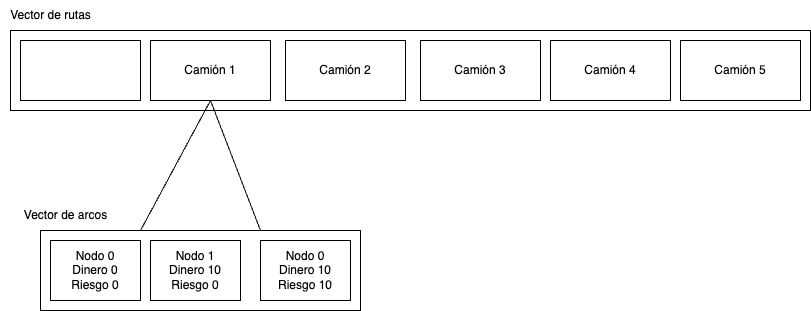
\includegraphics[scale = 0.5]{images/vectores.png}
        \label{fig: representación}
        \caption{Diagrama de la representación utilizada}
    \end{figure}
\end{center}

En el diagrama, el camión 1 tendría la ruta $0 \rightarrow 1 \rightarrow 0$. Esta representación es adecuada para el problema, ya que es extremadamente clara y facilita muchos de los cálculos. Por ejemplo, para calcular el riesgo total de un vehículo, basta con obtener el riesgo del último arco de cada camión, ya que tiene el riesgo acumulado. Además, se hace muy simple contar cuántos camiones son necesarios, ya que basta calcular el largo del vector de rutas. 

Para checkear las restricciones se hizo uso de un vector adicional, donde la casilla $i$ del vector contiene un 1 si es que el cliente $i$ ha sido ya visitado y un $0$ si es que no. Esta estructura adicional facilita mucho el chequeo de restricciones ya que por definición cada nodo solo será visitado una sola vez. Esto genera que muchas de las restricciones no tengan que ser implementadas como tal, ya que las estructuras utilizadas restringen las soluciones candidatas por definición. 

Por otro lado, con la representación del modelo matemático presentado anteriormente, se tenía la variable:
\begin{equation*}
    x^r_{ij}= 
    \begin{cases}
        1 & \text{si el arco $(i,j)$ es recorrido por el vehículo en la ruta r}\\
        0 & \text{en otro caso}
    \end{cases}
\end{equation*}
Esto, para $n$ clientes nos da un espacio de búsqueda de $2^{n \cdot |A|}$, donde $|A|$ es la cantidad de arcos totales del grafo. Dado que el grafo del problema es completo, se tiene que $|A| = n(n+1)/2$, lo que nos da un espacio de búsqueda total de $2^{n^2(n+1)/2}$. Ahora bien, con la representación utilizada para resolver el problema, se tiene un vector el cual fue explicado anteriormente. Para poder comprender de mejor manera el espacio de búsqueda que produce esta representación, podemos simplificarla. Si cada nodo es asignado a un camión (para que sea parte de su ruta), tenemos que el espacio de búsqueda es la cantidad de formas que podemos repartir $n$ clientes en a lo más $n$ camiones. Esto se puede ilustrar de la siguiente forma: la representación se puede reducir a un \texttt{string} simple de la forma: $$11110110111110...$$ donde cada conjunto de 1's representa la cantidad de clientes que lleva un camión en particular hasta llegar a un 0. Por ejemplo aquí en camión 1 llevaría los primeros 4 0's, el camión 2 los 2 1's que siguen, y así. Cabe notar que en este string es de largo total $2n-1$ y hay $n-1$ 0's. De esta forma, ahora para encontrar el espacio de búsqueda debemos encontrar la cantidad de maneras en las que se pueden distribuir los 0's. Esto es un problema de permutaciones conocido y tiene la forma: 
\begin{equation*}
    \binom{2n-1}{n-1} = \frac{(2n-1)!}{(n-1)!\cdot n!}
\end{equation*}

Luego, se puede evidenciar que:
\begin{equation*}
    \left(\left(\left(\sqrt{2}\right)^n\right)^n\right)^{n+1} > \frac{(2n-1)!}{(n-1)!\cdot n!}
\end{equation*}

Por lo que se reduce el espacio de búsqueda al utilizar esta representación. 
\newpage
\section{Descripci\'on del algoritmo}
Para resolver este problema se utilizó el algoritmo \textit{Hill Climbing First Improvement}. Este algoritmo corresponde a una técnica incompleta de búsqueda, cuya estructura se puede apreciar a continuación:
\begin{algorithm}
    \caption{Hill Climbing Alguna Mejora}\label{alg:cap}
    \begin{algorithmic}
        \State $local \gets FALSE$
        \State $s_c \gets \text{select a point at random}$
        \State $neighbor \gets 0$
        \Repeat
        \State $s'_n \gets \text{generate a neighbor point in } \mathscr{N}(s_c)$
        
        $neighbor++$
        \If{$f(s'_n)$ is better than $f(s_c)$}
            \State $s_c \gets s'_n$
            \State $neighbor \gets 0$
        \EndIf
        \If{neighbor == max\_neighbors}
            \State $local \gets TRUE$
        \EndIf
        \Until{local}
    \end{algorithmic}
\end{algorithm}

Este algoritmo requiere de dos componentes para su realización. Primero se requiere una solución inicial y un movimiento para generar un vecindario. Para esta resolución del problema, la solución inicial fue generada por un algoritmo \textit{Greedy}, y el movimiento consistirá en un intercambio de clientes entre camiones.

\subsection{Generación de solución inicial}
Como se mencionó anteriormente, la generación de la solución inicial que se utilizó en el algoritmo fue obtenida con un algoritmo \textit{Greedy}. Para medir la calidad de las soluciones se utilizó una función de evaluación que suma la distancia total de todos los camiones. Esto se debía minimizar, como fue indicado en el modelo matemático. Para generar la solución, el \textit{Greedy} implementado fue basado en la técnica Clarke-Wright \cite{clarke1964scheduling}, la cual consiste en iniciar con un camión por cada cliente, y luego iterar por todos los pares de rutas y ver si es que mejora la calidad al combinarlas. Esto se puede apreciar mejor a continuación:

\begin{minipage}{0.5\textwidth}
    \begin{figure}[H]
        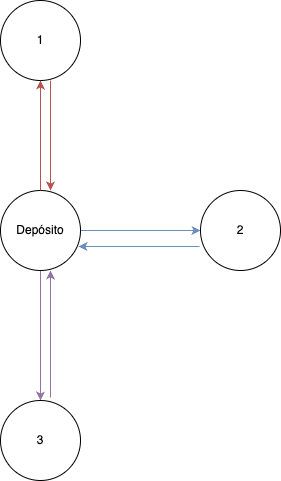
\includegraphics[scale = 0.3]{images/greedy.png}
        \label{fig: inicial}
        \caption{Estado inicial}
    \end{figure}
\end{minipage}
\begin{minipage}{0.5\textwidth}
    \begin{figure}[H]
        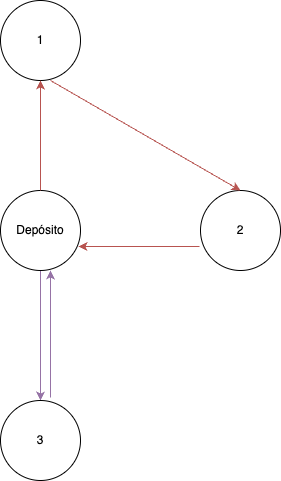
\includegraphics[scale = 0.3]{images/greedy2.png}
        \label{fig: merge}
        \caption{Juntar dos rutas}
    \end{figure}
\end{minipage}

\subsection{Movimiento}
El movimiento utilizado en la solución del problema, consiste en intercambiar los clientes de un camión con un subconjunto de clientes de otro camión. Este movimiento fue inspirado por una implementación de Hill Climbing para un VRP por Souza y Chagas \cite{souza2020late} y fue elegido dado que no es muy complejo de implementar y genera un vecindario que involucra las rutas de todos los camiones. Por ejemplo, si se tiene la siguiente solución candidata:

\begin{figure}[H]
    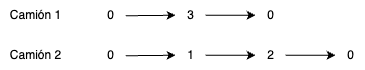
\includegraphics[scale = 0.5]{images/sol.png}
    \label{fig: candidatesol}
    \caption{Solución candidata}
\end{figure}

Se tiene el siguiente vecindario:
\begin{figure}[H]
    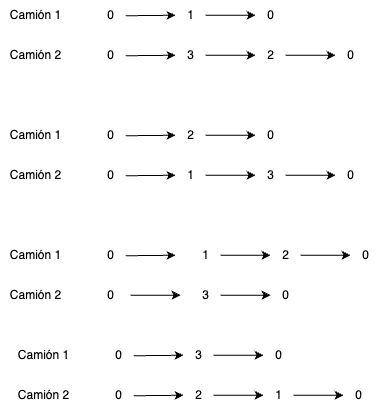
\includegraphics[scale = 0.5]{images/vecindario.png}
    \label{fig: neighborhood}
    \caption{Vecindario producido al aplicar el movimiento}
\end{figure}

Esto es porque los subconjuntos formados por los clientes del camión 2 corresponden a $\left\{1\right\}, \left\{2\right\}, \left\{1,2\right\}$, por lo que el cliente 1 del camión 1 se intercambia con cada uno de esos subconjuntos. Cabe mencionar que si el camión 1 tuviera más de un cliente, los intercambios se harían con ese cliente también.

\subsection{Implementación del algoritmo}
Teniendo la solución inicial y el movimiento definido, para la implementación del algoritmo lo primero que se realizó fue una función que generara un vecino en específico, que sea factible, es decir, se checkea que cumplan las restricciones antes de considerarlo como un vecino como tal. Luego, se itera por todos los camiones de la solución candidata, para luego iterar por cada cliente de cada camión. Una vez que se tiene un cliente que va a ser intercambiado, nuevamente se itera por todo el resto de los camiones para luego obtener los subconjuntos con los cuales va a ocurrir el intercambio. Posteriormente se genera cada vecino con los subconjuntos obtenidos, hasta lograr una mejora. En caso de que la haya, esa se convierte en la mejor solución candidata. El algoritmo termina cuando no encuentre ninguna mejora. 

\begin{algorithm}[H]
    \caption{Hill Climbing Alguna Mejora: Implementación para este problema}\label{alg:cap1}
    \begin{algorithmic}
        \State $local \gets true$
        \While{$local$}
            \State $c_i \gets \text{current quality}$
            \State $update \gets false$
            \For{each truck available}
                \For{each client in truck}
                    \For{each other truck available}
                        \State generate subsets
                        \If{neighbor(subset) is feasible}
                            \State $c_n \gets \text{new quality}$
                            \If{$c_i > c_n$}
                                \State $c_i \gets c_n$
                                \State $update \gets true$
                            \EndIf
                        \EndIf
                    \EndFor
                \EndFor
            \EndFor
            \State $local \gets update$
        \EndWhile
    \end{algorithmic}
\end{algorithm}

\newpage
\section{Experimentos}
Para realizar los experimentos, se cuenta con 4 sets de instancias para probar el funcionamiento del algoritmo, de las cuales se testearán 3 instancias de cada uno. En cada instancia se entrega la cantidad de clientes que deben ser atendidos, el riesgo máximo permitido, y las coordenadas de cada nodo incluyendo el depósito. El fin de no haber probado con todas las instancias proporcionadas es poder hacer un estudio inicial con respecto a otros trabajos realizados. Por ejemplo, Talarico \cite{talarico2015metaheuristics} prueba con una cantidad similar de instancias. Además, probar todas las instancias proporcionadas implicaría un consumo de tiempo considerable y no tiene beneficios tangibles dado que en la literatura no se suele probar con semejante cantidad. Las características de los sets elegidos para los experimentos al igual que las instancias que contienen se pueden ver resumidos a continuación:
\begin{table}[H]
    \centering
    \begin{tabular}{|c|c|c|c|}
    \hline
    Instancia      & Set & Cantidad nodos & Nivel de Riesgo \\ \hline
    10.txt         & O   & 10             &                 \\ \hline
    55.txt         & O   & 55             &                 \\ \hline
    81.txt         & O   & 81             &                 \\ \hline
    51.txt         & V   & 51             & 1.0             \\ \hline
    121.txt        & V   & 121            & 1.0             \\ \hline
    51.txt         & V   & 51             & 1.5             \\ \hline
    121.txt        & V   & 121            & 1.5             \\ \hline
    51.txt         & V   & 51             & 2.0             \\ \hline
    121.txt        & V   & 121            & 2.0             \\ \hline
    51.txt         & V   & 51             & 2.5             \\ \hline
    121.txt        & V   & 121            & 2.5             \\ \hline
    51.txt         & V   & 51             & 3.0             \\ \hline
    121.txt        & V   & 121            & 3.0             \\ \hline
    12\_7\_1.0.txt & R   & 12             & 1.0             \\ \hline
    20\_7\_1.0.txt & R   & 20             & 1.0             \\ \hline
    12\_7\_1.5.txt & R   & 12             & 1.5             \\ \hline
    20\_7\_1.5.txt & R   & 20             & 1.5             \\ \hline
    12\_7\_2.0.txt & R   & 12             & 2.0             \\ \hline
    20\_7\_2.0.txt & R   & 20             & 2.0             \\ \hline
    12\_7\_2.5.txt & R   & 12             & 2.5             \\ \hline
    20\_7\_2.5.txt & R   & 20             & 2.5             \\ \hline
    12\_7\_3.0.txt & R   & 12             & 3.0             \\ \hline
    20\_7\_3.0.txt & R   & 20             & 3.0             \\ \hline
    25.txt         & S   & 25             &                 \\ \hline
    40.txt         & S   & 40             &                 \\ \hline
    64.txt         & S   & 64             &                 \\ \hline
    \end{tabular}
    \caption{Información sobre instancias}
    \label{tab:info_instances}
\end{table}


Para el hardware de los experimentos se utilizó un MacBook Air M1 2020 con sistema operativo Sonoma 14.1.1. La CPU utilizada es un Apple M1 con 68.3 [GB/s]

\newpage
\section{Resultados}
Para presentar los resultados se tendrá la calidad de la solución inicial generada por \textit{Greedy}, la calidad luego de aplicar \textit{Hill Climbing}, el porcentaje de mejora obtenido y el tiempo de ejecución de cada instancia.

A continuación se presentan los resultados obtenidos:
\begin{table}[H]
    \small
    \begin{tabular}{|c|c|c|c|c|c|c|c|}
    \hline
    Instancia     & Instancia      & Set & Cantidad nodos & Calidad Greedy & Calidad HCAM & Tiempo \{s\} & Mejora \\ \hline
    O: 10.txt     & 10.txt         & O   & 10             & 314,159        & 268,324      & 0,007796     & 15\%   \\ \hline
    O: 55.txt     & 55.txt         & O   & 55             & 205,787        & 125,664      & 205032       & 39\%   \\ \hline
    O: 81.txt     & 81.txt         & O   & 81             & 286,802        & 198,357      & 33,5822      & 31\%   \\ \hline
    V:1.0 121.txt & 121.txt        & V   & 121            & 1859,15        & 1531,25      & 11,8684      & 18\%   \\ \hline
    V:1.0 51.txt  & 51.txt         & V   & 51             & 6680,38        & 6248,4       & 113,64       & 6\%    \\ \hline
    V:1.5 51.txt  & 51.txt         & V   & 51             & 1591,37        & 1215,28      & 167,495      & 24\%   \\ \hline
    V:1.5 121.txt & 121.txt        & V   & 121            & 4699,05        & 4197,13      & 268,429      & 11\%   \\ \hline
    V:2.0 51.txt  & 51.txt         & V   & 51             & 1644,67        & 1046,02      & 181,232      & 36\%   \\ \hline
    V:2.0 121.txt & 121.txt        & V   & 121            & 3743,07        & 3189,35      & 655,202      & 15\%   \\ \hline
    V:2.5 51.txt  & 51.txt         & V   & 51             & 1554,6         & 942,716      & 22,8449      & 39\%   \\ \hline
    V:2.5 121.txt & 121.txt        & V   & 121            & 3181,01        & 2842,48      & 1375,93      & 11\%   \\ \hline
    V:3.0 51.txt  & 51.txt         & V   & 51             & 1567,01        & 863          & 4,54328      & 45\%   \\ \hline
    V:3.0 121.txt & 121.txt        & V   & 121            & 2977,67        & 2376,55      & 3633,68      & 20\%   \\ \hline
    R:1.0 12 7    & 12\_7\_1.0.txt & R   & 12             & 1387,99        & 1387,99      & 0,013359     & 0\%    \\ \hline
    R:1.0 20 7    & 20\_7\_1.0.txt & R   & 20             & 1208,29        & 1091,65      & 0,052268     & 10\%   \\ \hline
    R:1.5 12 7    & 12\_7\_1.5.txt & R   & 12             & 1131,01        & 955          & 0,010628     & 16\%   \\ \hline
    R: 1.5 20 7   & 20\_7\_1.5.txt & R   & 20             & 1241,27        & 987,02       & 0,068965     & 20\%   \\ \hline
    R:2.0 12 7    & 12\_7\_2.0.txt & R   & 12             & 984,402        & 782,345      & 0,015343     & 21\%   \\ \hline
    R:2.0 20 7    & 20\_7\_2.0.txt & R   & 20             & 1051,82        & 819,52       & 0,051811     & 22\%   \\ \hline
    R:2.5 12 7    & 12\_7\_2.5.txt & R   & 12             & 988,907        & 739,355      & 0,015741     & 25\%   \\ \hline
    R: 2.5 20 7   & 20\_7\_2.5.txt & R   & 20             & 1015,91        & 721,257      & 0,043044     & 29\%   \\ \hline
    R:3.0 12 7    & 12\_7\_3.0.txt & R   & 12             & 795,603        & 571,079      & 0,016201     & 28\%   \\ \hline
    R:3.0 20 7    & 20\_7\_3.0.txt & R   & 20             & 1002,64        & 728,94       & 0,059606     & 27\%   \\ \hline
    S: 25.txt     & 25.txt         & S   & 25             & 66,3587        & 55,8583      & 0,091152     & 16\%   \\ \hline
    S: 40.txt     & 40.txt         & S   & 40             & 162,863        & 160,216      & 0,889194     & 2\%    \\ \hline
    S: 64.txt     & 64.txt         & S   & 64             & 282,356        & 282,356      & 375,6          & 0\%    \\ \hline
    \end{tabular}
    \caption{Resultados obtenidos}
    \label{tab:results}
    \end{table}

    Se puede ver que a partir de 64 nodos en adelante, el tiempo aumenta bastante. Las instancias de más de 100 nodos se podían llegar a demorar 1 hora en terminar de ejecutarse. Esto se debe a que el movimiento genera un vecindario que aumenta exponencialmente con la cantidad de nodos, porque revisa si se puede intercambiar con todos los subconjuntos posibles. Sin embargo, hubo una cantidad no menor de casos donde se vieron mejoras considerables respecto a la solución generada por \textit{Greedy}, con hasta un 45\% de mejora. 
\newpage
\section{Conclusiones}
El problema VRP es un problema extremadamente estudiado, y cuenta con una gran cantidad de variantes. Específicamente, la variante de RCVRP es una compleja variación debido a todas sus restricciones. Este estudio ha tomado en cuenta la naturaleza NP-hard del problema y la necesidad de aplicar heurísticas y metaheurísticas en lugar de técnicas que aseguren una solución óptima. 

Para instancias de tamaño pequeño, la combinación de los algoritmos \textit{Greedy} y \textit{Hill Climbing First Improvement} ha demostrado bastante eficacia, ofreciendo mejoras significativas en poco tiempo. Sin embargo, al aumentar la cantidad de nodos el tiempo aumenta exponencialmente. Esto se debe principalmente al movimiento elegido y además a la naturaleza del problema, pues el grafo siempre es completo y eso aumenta considerablemente las posibilidades de rutas. Por esta razón esta implementación es bastante limitada por la cantidad de clientes, y no sería factible utilizarla en problemas de gran escala. 

La relevancia destacada de este estudio destaca en el logro de una implementación correcta de los algoritmos \textit{Greedy} y \textit{Hill Climbing First Improvement}. Esta implementación ha demostrado ser particularmente eficiente en instancias de pequeña escala, donde se han observado mejoras sustanciales en la calidad de las soluciones con tiempos de ejecución reducidos.

Como trabajo futuro se podría realizar un estudio sobre algún movimiento que permita mejorar los tiempos de ejecución sin sacrificar las posibilidades de rutas que se puedan generar. De la misma manera, se podría buscar cómo adaptarlo a situaciones de la vida real, añadiendo más restricciones y podando así el espacio de búsqueda.

\newpage
\bibliographystyle{unsrt}
\small
\bibliography{Referencias}

\end{document} 
